\documentclass{article}
\usepackage[utf8]{inputenc}
\usepackage[margin=1.0in]{geometry}
\usepackage{graphicx}
\usepackage{wrapfig}
\usepackage{amsmath}
\usepackage[makeroom]{cancel}
\let\vec\mathbf

\title{Classification Models}
\author{Alexey Didenkov, George Tang}
\date{December 5, 2018}

\begin{document}

\maketitle

\section{Introduction}
Today is the day that we finally dip our toes into the complex and broad field of Machine Learning. While ML does not directly relate to computer vision, the two fields often overlap - machine learning models can be used to aid the task of computer vision, and plenty of ML is focused on cracking the problem of computer vision through new and more powerful architectures. The approaches they take often differ - in general, CV focuses on rigorous manually-written code, while ML aims to create networks that can interpret large amounts of data and learn the problem themselves. Each has its own strengths and weaknesses, and it's important to know which contexts suit each of them best to utilize them most efficiently.
\subsection{Machine Learning}
\textbf{Machine Learning} is the study of computer algorithms and models that \textit{progressively improve} their performance on a specific task. It's this continuous improvement that we call \textbf{learning}. It should be noted that most present approaches focus on solving specific tasks and utilizing large amounts of data.
\subsection{Types}
There are several main types of machine learning:
\begin{itemize}
    \item \textbf{Supervised learning} solves problems that provide \textbf{both} the data and its ground-truth labels
    \item \textbf{Unsupervised learning} deals with data that has \textbf{no labels}
    \item \textbf{Reinforcement learning} explores how agents behave in an environment
\end{itemize}
These act as the tree main branches of ML. Since the problems that belong to different groups differ, so do the models that try to solve them. Note that of the four algorithms we are about to discuss, one (k-means) belongs to a different group (Unsupervised learning) than the other three.
\subsection{Traditional ML}
The algorithms we are about to discuss today are often presently labeled as \textbf{traditional ML}. This does not imply that these models are bad or outdated, and is more of a term to distinguish them from the other existing kind, \textbf{deep learning}. The latter of the two focuses on building more complex models that perform better, yet it still owes many of its fundamental building blocks to traditional ML. We'll explore deep learning further in the next week's lecture.

\section{Decision trees}
\subsection{Problem type}
Imagine that we have some points that lie on the x-y plane. All of these points have a number assigned to them, also known as their \textbf{label}. This is the number we want our network to predict, thus making the task fall under \textbf{supervised learning}.
\begin{figure}[!htb]
    \begin{center}
        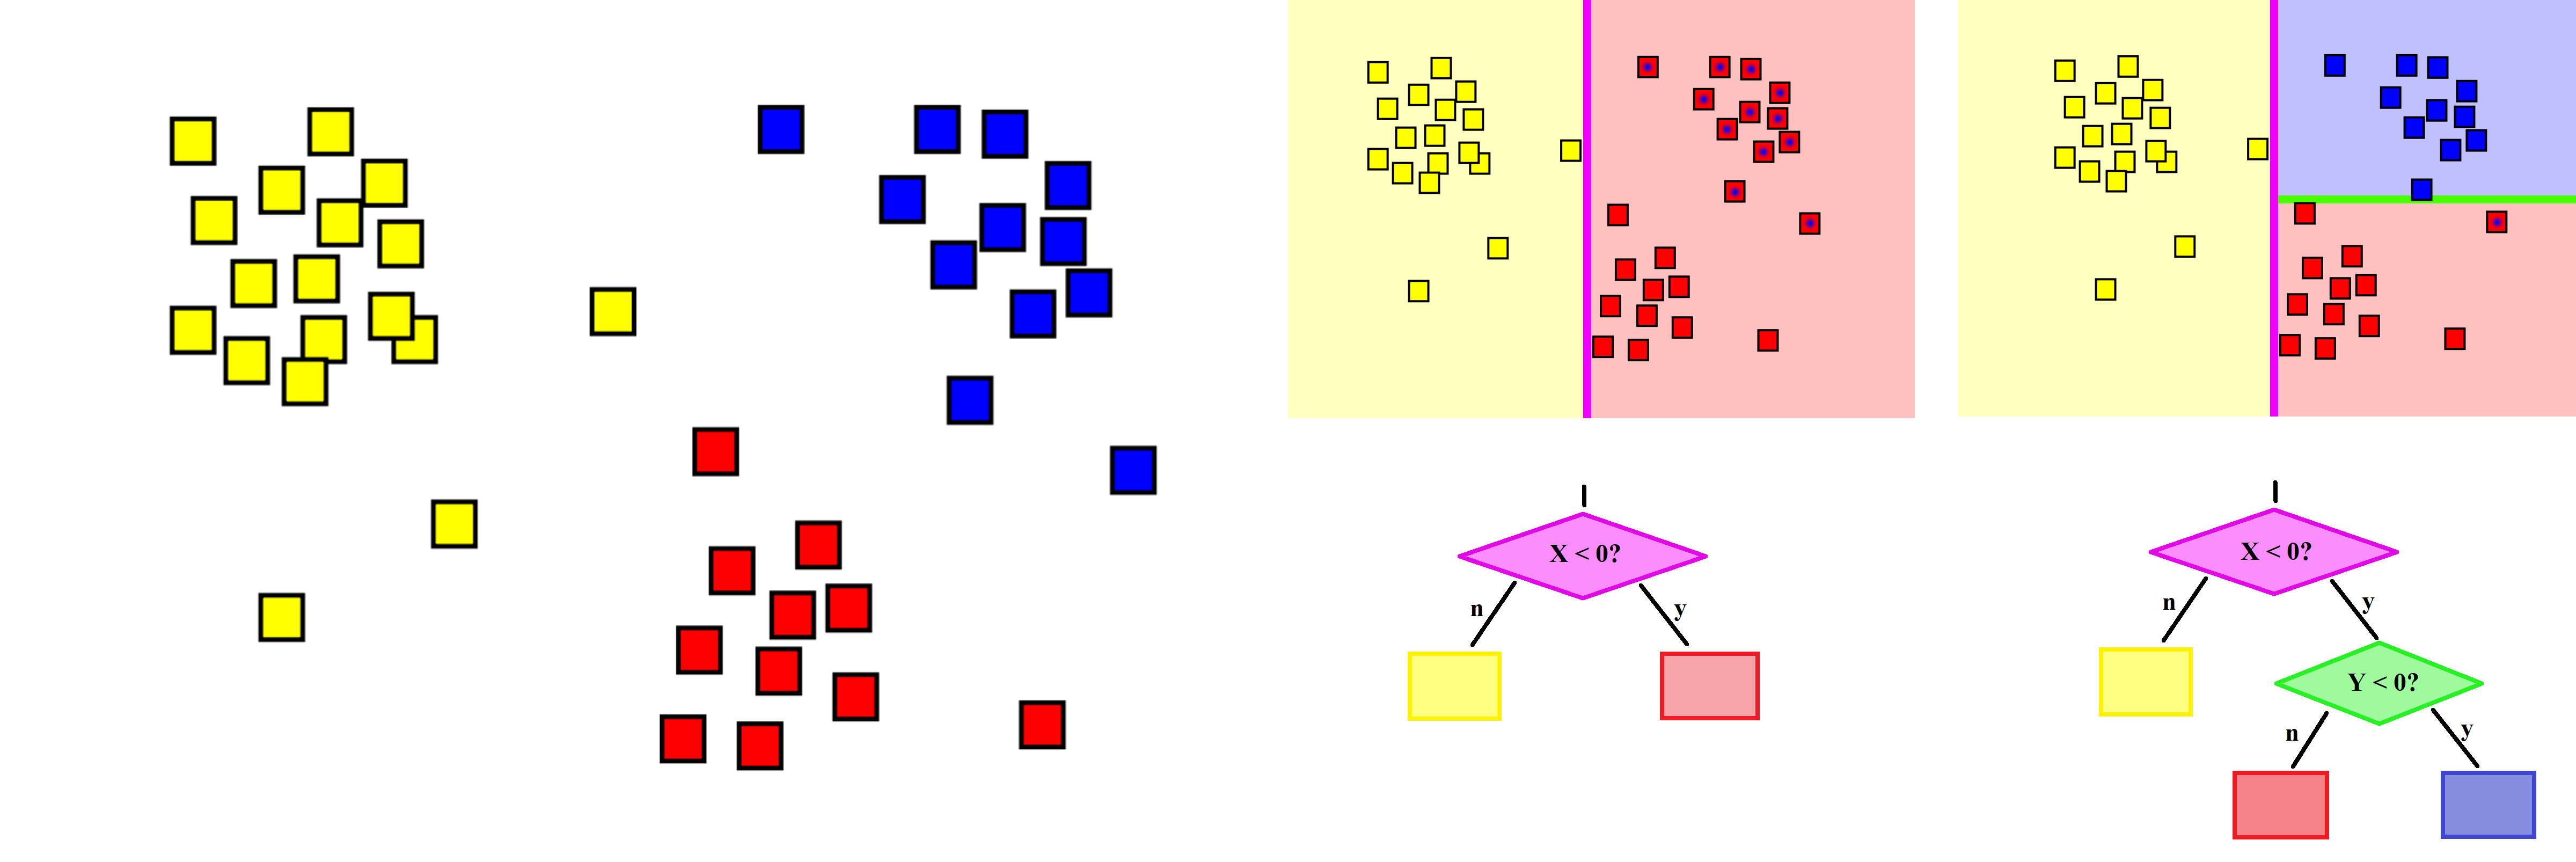
\includegraphics[width=0.9\textwidth]{combined.png}
    \end{center}
    \vspace{-10pt}
    \caption{Simple decision tree example}
\end{figure}
\subsection{Decision trees}
What we can do now is start slicing the x-y plane in an attempt to separate the points. We make every such cut along a single variable, finding a threshold value, and placing everything under that threshold in one category, and everything greater into an another. We can represent this in tree form, and continue further breaking down the resulting regions.

\begin{wrapfigure}{r}{0.35\textwidth}
  \begin{center}
    \vspace{-60pt}
    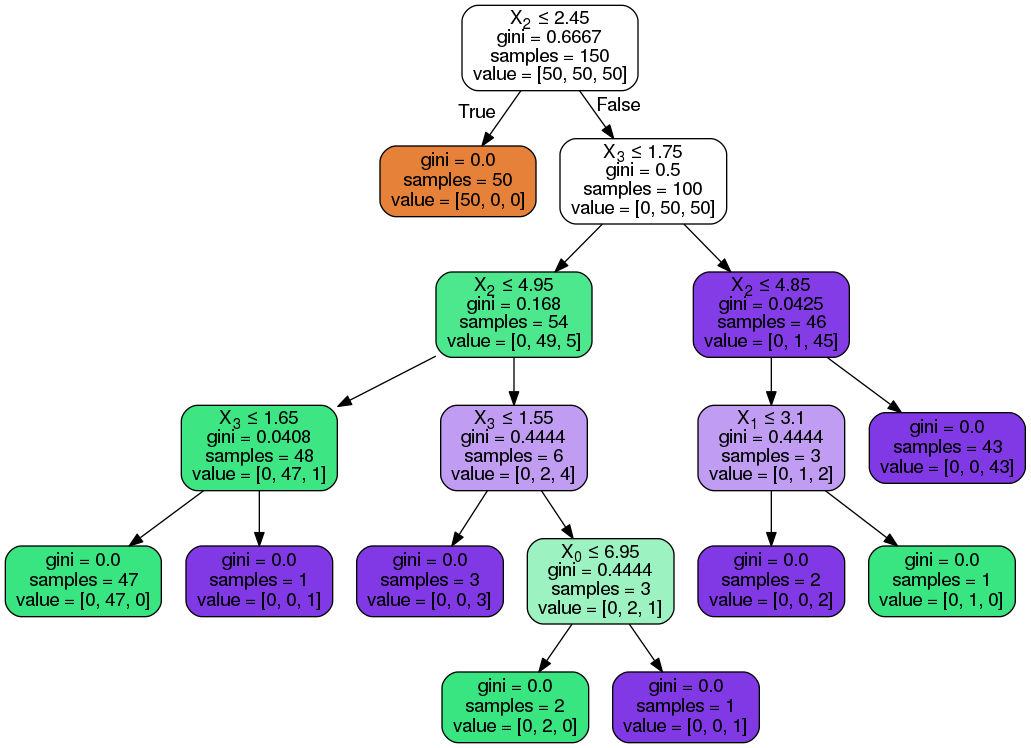
\includegraphics[width=0.35\textwidth]{DecisionTree.png}
    \vspace{-35pt}
  \end{center}
  \caption{A larger decision tree, fit on real data}
  \vspace{-35pt}
\end{wrapfigure}

\subsection{Splitting}
Our goal is to separate the points so no labeled group shares the same region with points of another label. This creates a \textit{prediction model}, allowing us to take an unknown point, traverse the tree, and determine the point's label. How do we choose where to split the region (threshold)? We want to maximize the \textbf{information gain}:
\\
\\
\begin{left}
\hspace{40pt}
$$ IG(D) = I(D) - \frac{N_{left}}{N}I(D_{left}) - \frac{N_{right}}{N}I(D_{right}) $$
\end{left}
\\
\\
\\
where $D$ is the node, $N$ is the number of elements, and $I$ is the \textbf{impurity}. It has a score of 0 for regions whose points belong to only one label, and gets closer to 1 otherwise. Essentially by maximizing the information gain, we find a split such that the impurity of the resulting children is minimum. It can be defined in multiple ways. Below are the \textbf{entropy} and \textbf{Gini Impurity}, respectively:

$$ I_H(D) = - \sum_{i=1}^{c} p(i|D)\log_2p(i|D) \mid c \neq \emptyset $$
$$ I_G(D) = 1 - \sum_{i=1}^{c} p(i|D)^2 $$ 
\noindent
where $c$ is the number of classes and $p(i|D)$ is the probability of class $i$ occurring in node $D$ (number of elements in $c$ over total elements).

\subsection{Random Forests}
A powerful feature of trees comes from how computationally simple they are. So, a common practice with trees is to create many slightly different versions, in what is known as a \textbf{random forest}. Even if a single tree is likely to mess up, the case is not so with an entire forest - congregating the results of several models typically provides a more reliable result overall.

\section{SVMs}
\begin{wrapfigure}{r}{0.2\textwidth}
  \begin{center}
    \vspace{-35pt}
    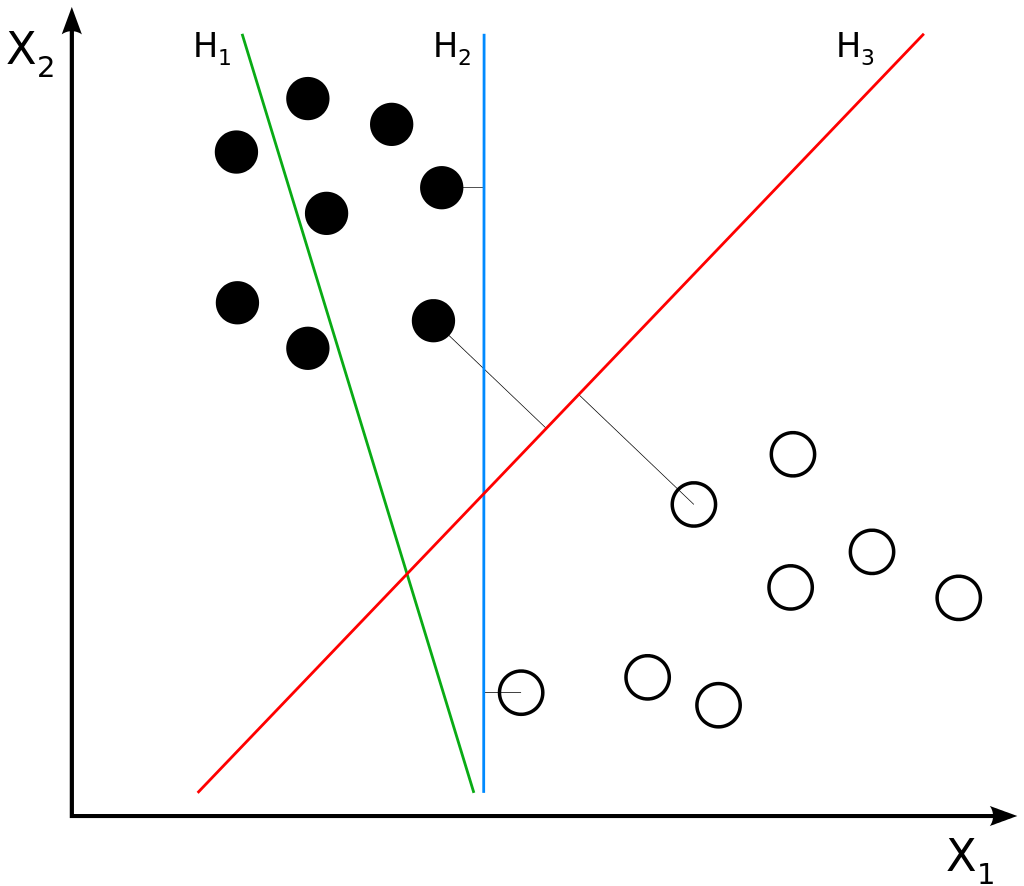
\includegraphics[width=0.2\textwidth]{SVMseparate.png}
    \vspace{-30pt}
  \end{center}
  \caption{Several potential separations}
  \vspace{-10pt}
\end{wrapfigure}
Imagine that we have the same type of data, but now our data is not easily separable by vertical or horizontal lines-  it requires a slanted line, one that considers both x and y. While decision trees could achieve this by making a zigzagged-line, this is computationally inefficient and would produce a very large and deep tree. We desire a solution that's capable of making such cuts intrinsically.

Additionally, there are often multiple cuts that can separate the data in an identical way. On Figure 3, the blue vertical line partitions the data exactly like the red diagonal one does, yet the former works way worse as a prediction model. The reason being that it \textbf{cuts dangerously close} to the real data - black points slightly further to the right and white ones slightly over to the left would both get classified incorrectly.

\subsection{Support Vector Machines}
\begin{wrapfigure}{r}{0.25\textwidth}
  \begin{center}
    \vspace{-60pt}
    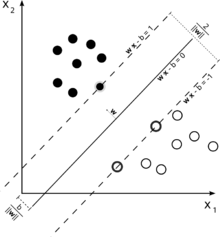
\includegraphics[width=0.25\textwidth]{separateMargin.png}
    \vspace{-30pt}
  \end{center}
  \caption{Separation with a margin}
  \vspace{-30pt}
\end{wrapfigure}
if we only looked at homogeneity/accuracy we wouldn't be able to detect the subtlety of these differences. Introducing: support vectors. On each side of the line, we draw a perpendicular vector to the closest point of the respective class. These become the \textbf{support vectors}, their combined length measuring the width of the margin. We can rely on these support vectors to make our separation more robust by changing it to maximize the sum of the vectors' lengths.

\subsection{Linear classification}
We can write the equation of the hyperplane as
$$ \vec{w} \cdot \vec{x} - b=0 $$
where $w$ is the vector normal to the hyperplane and $x$ is the position vector in the feature space $x_1, x_2, x_3$ ... The top and bottom lines parallel to the hyperplane defined by the support vectors and the distance between them can be thus defined as
$$ \vec{w} \cdot \vec{x} - b=1 $$
$$ \vec{w} \cdot \vec{x} - b=-1 $$
$$ distance = \frac{2}{||w||}$$
Moreover, we have the constraint that no points must be within the gap defined by the support vectors, which can be mathematically expressed as
$$ y(\vec{w} \cdot \vec{x} - b) \geq 1$$ 
where $y$ is -1 for points below the line and 1 for above. We want the maximize the distance or minimize $||w||$ given the constraint, which can be reformulated as a \textbf{Lagrange Multiplers} problem (consults Resources section on website for math).

\subsection{Nonlinear classification}
So far, we've been separating the data with \textbf{straight lines}. Even those separations that depend on multiple variables are characterized by their \textit{linearity} - they retain that property no matter how many variables they consider, no matter if they are a line, a plane, or a hyperplane.

What if our data looked like a circle on the plane, where everything inside that circle as part of one class and everything outside of another. Surely, it would help if we could draw circles instead of lines to separate the points.
\begin{figure}[!htb]
    \vspace{-10pt}
    \begin{center}
        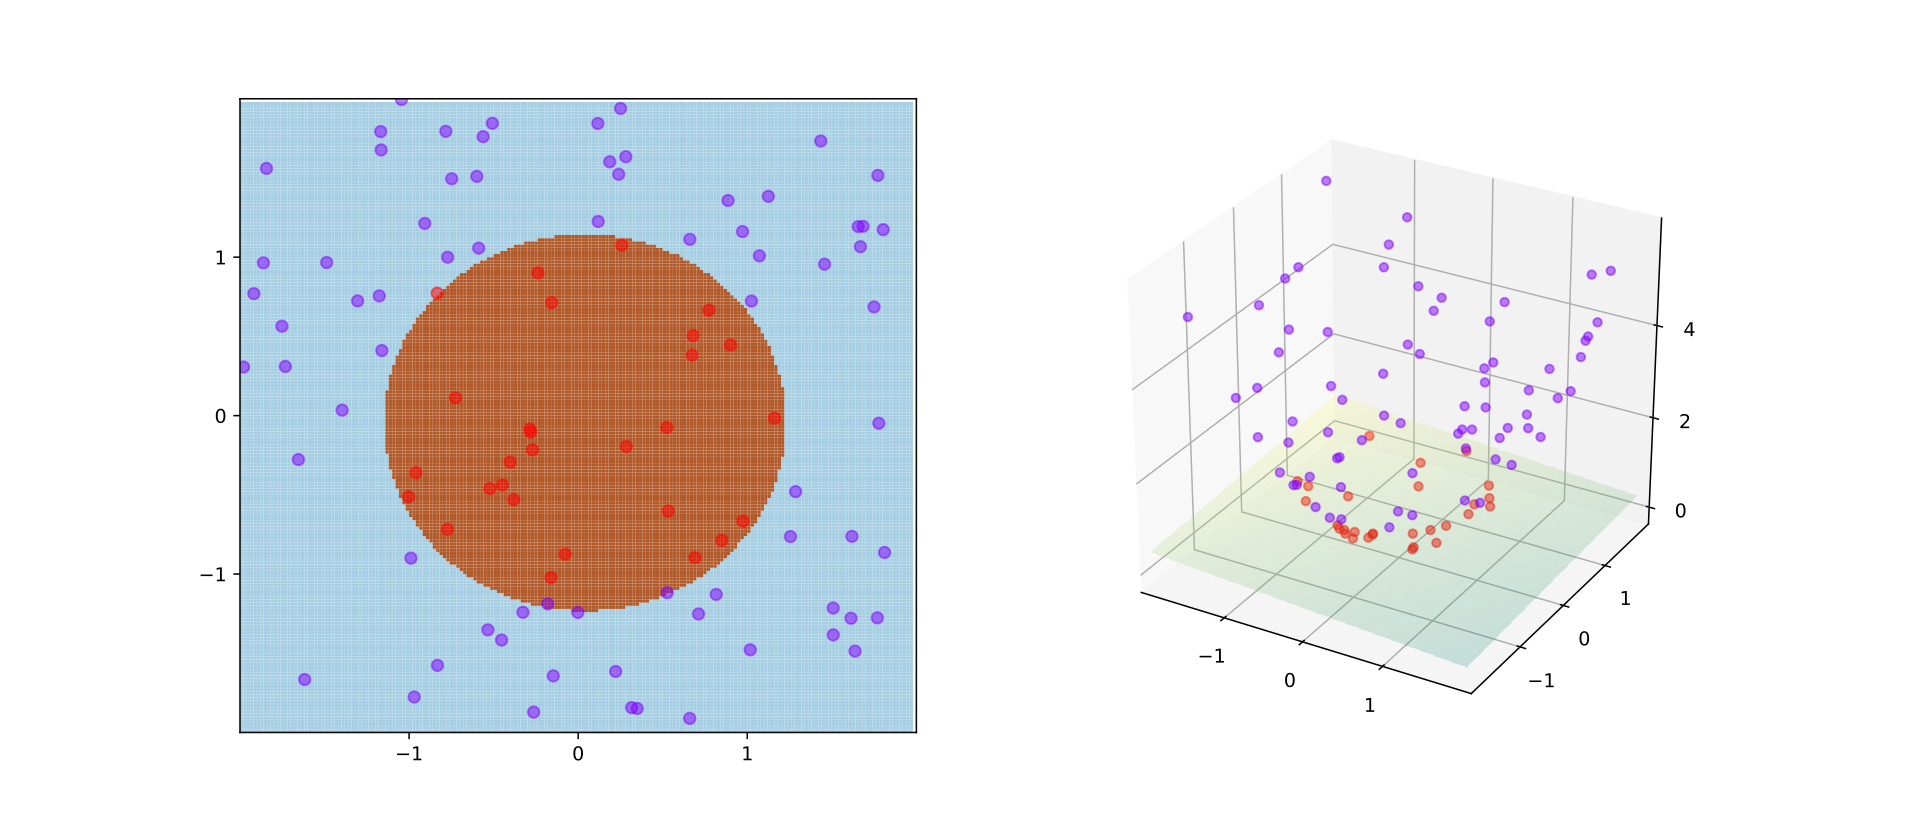
\includegraphics[width=0.8\textwidth]{kernel.png}
    \end{center}
    \vspace{-25pt}
    \caption{SVM with a kernel}
    \vspace{-10pt}
\end{figure}

Our solution, then, is to calculate the distance from the origin, $z = r^2 = x^2 + y^2$, and feed that in as a third parameter along with $x$ and $y$. Used in this context, the function becomes a \textbf{kernel function}. The resulting points look identical when viewed from above, but they now lie on the surface of a paraboloid. Separating the circle now becomes easy - drawing a $z = k$ plane becomes identical to drawing a circle with radius $\sqrt{k}$.

\begin{wrapfigure}{r}{0.3\textwidth}
  \begin{center}
    \vspace{-25pt}
    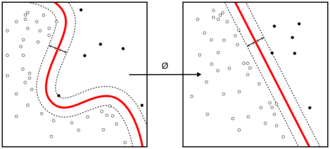
\includegraphics[width=0.29\textwidth]{kernel-transform.png}
    \vspace{-20pt}
  \end{center}
  \caption{Kernels transforming feature space}
  \vspace{-20pt}
\end{wrapfigure}
It should be noted that real SVMs usually implement kernels a bit differently. They define hyperplanes using the support vectors and the \textit{dot product}, the latter of which can be redefined from its normal definition to implement this kernel functionality. That's also why kernels are sometimes thought of as transforming the feature space, so that our separations actually look like straight lines.

\section{K-nearest neighbors (KNN)}
Like decision trees and SVMs, K-nearest neighbors (a.k.a KNN) is a \textbf{supervised learning} method and focuses on predicting class labels based on given labeled data. However, unlike the previous two, KNN does not create definite partitions of space based on global data, and instead uses \textbf{local} data, i.e. nearby \textbf{neighbors}, to predict labels.

\begin{wrapfigure}{r}{0.25\textwidth}
  \begin{center}
    \vspace{-40pt}
    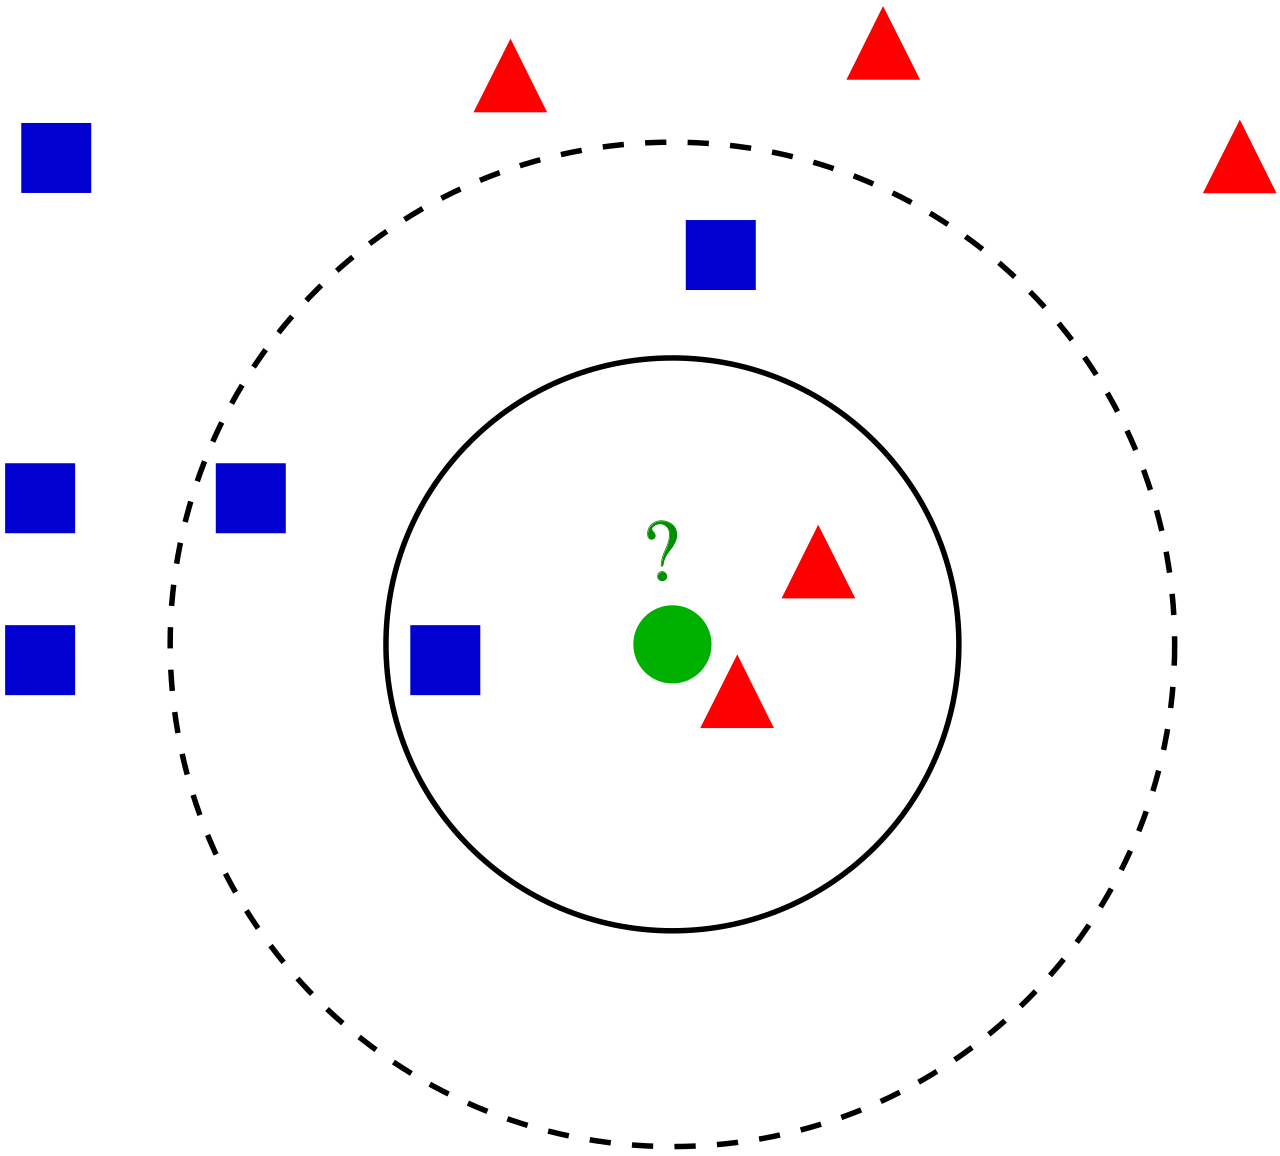
\includegraphics[width=0.25\textwidth]{KNN.png}
    \vspace{-30pt}
  \end{center}
  \caption{Two different choices of K for KNN yeild different results.}
  \vspace{-30pt}
\end{wrapfigure}

\subsection{Classification}
In classification, we begin with a labeled data set in a feature space. When we are given an unlabeled data set, the K nearest neighbors vote on its classification. In other words, it is labeled as the most commonly occurring label in the K-nearest neighbors. When we only use the nearest point, it is known as the \textbf{1-nearest neighbor classification}. We can also weigh the K-nearest neighbors, considering closer points as more important according to $L_1$ or $L_2$, for instance (mean absolute error and mean squared error). You can think of them as the 'distance' to the unlabeled data point in feature space.

\subsection{Regression}
In regression, KNN uses the K nearest neighbors' statistical properties to determine a statistical value for the unlabeled point. Often, it is simply the average of the KNN, or it can be likewise weighted.

\subsection{K selection}
Larger values of K reduce noise, but can also lead to consideration of irrelevant features. Smaller values of K lead to noise. Both can severely hinder the performance of the algorithm. There is much research in manipulating features, such as scaling or selecting certain features, to improve accuracy.

\section{K-means clustering}

\subsection{Problem type}
Recall that in the beginning of the lecture we covered three types of machine learning and briefly mentioned that k-means belongs to a different type than the other two. Well, now it's time to elaborate on that. K-means clustering is an \textbf{unsupervised learning} that happens to be named similarly to K-nearest neighbors.

Think of the same points on a plane that we worked with previously. However, now there's a big difference - \textit{we don't have ground-truth label data}. We're stuck finding a model that separates the points without knowing which points should actually belong to different categories - we need to infer that from the overall structure of out points.

Why do we need to deal with such a problem? As it turns out, labeled data often happens to be fairly expensive. Unless it was already taken in an organized setting (such as patients with and without cancer, their data separated and labeled), labels don't exist on raw data and need to be made by experts (which is really expensive). Often, we end up relying on algorithms that don't need any labels, using the small amount that we do have to periodically \textbf{validate} how our network is doing, hence \textbf{unsupervised learning}.

\subsection{Clustering}
\begin{figure}[!htb]
    \vspace{-10pt}
    \begin{center}
        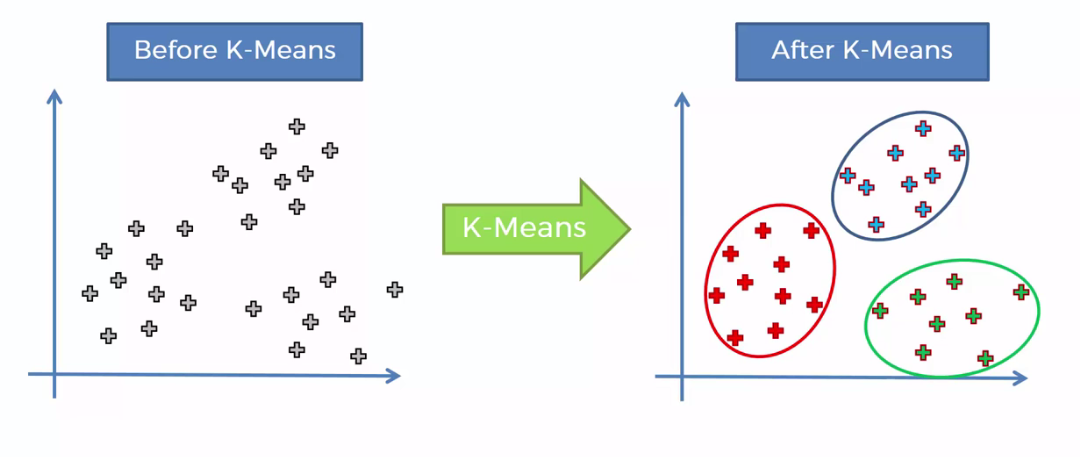
\includegraphics[width=0.6\textwidth]{kmeans.png}
    \end{center}
    \vspace{-30pt}
    \caption{Clustering example}
    \vspace{-10pt}
\end{figure}
Probably the most common type of unsupervised learning is cluster analysis, or \textbf{clustering}. The approach assumes that our data consists of \textit{several groups}, with members more similar to others within their same group and dissimilar to members of other groups. The goal of the approach is then to somehow find these groups.

There exists various algorithms that implement clustering, mainly differing by how they represent the clusters and how they find them. Some are more complex than others, but there isn't necessarily a "best method" that outperforms all others. Context is important, for example, a method that specifically deals with clusters of elongated and twisted shapes will perform way better when confronted with that kind of data, but may be outperformed by the most basic of algorithms when dealing with simple, circular clusters.

\subsection{K-means}
\textbf{K-means} is one such clustering algorithm. It represents clusters through their \textbf{centers} (a.k.a. means, centroids), and finds the optimum solution iteratively. To calculate which cluster a point belongs to, it finds the closest cluster center, meaning that:

\begin{wrapfigure}{r}{0.2\textwidth}
  \begin{center}
    \vspace{-77pt}
    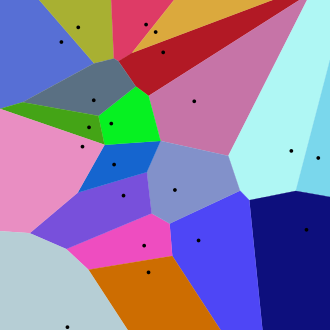
\includegraphics[width=0.2\textwidth]{voronoi.png}
    \vspace{-32pt}
  \end{center}
  \caption{Voronoi}
  \vspace{-27pt}
\end{wrapfigure}
\begin{minipage}{.75\textwidth}
    \vspace{2pt}
    \begin{enumerate}
        \item K-means works best with \textit{circular clusters} of \textit{equal size} - because distances from each cluster center are considered equally, the lines of separation get drawn an equal distance from each. Thus, big clusters will often have their points attributed to nearby smaller clusters.
        \item K-means is a \textbf{linear method} - the lines separating two clusters are straight and perpendicular to the lines that connect cluster centers, intersecting them at their midpoints. The resulting partitioning is also called a \textbf{Voronoi diagram}
    \end{enumerate}
\end{minipage}

K-means starts with $k$ random centers, or means, (hence the name), and finds its solution iteratively. It relies on the subtle difference between its cluster centers and the true means (or centroids) of the data within each cluster. The two values differing is sort of like getting different mean and median values, both imply that the data is \textit{skewed}, or heavy on one side versus another. In our situation, that probably means that the current cluster center is not at its true center, and so the algorithm updates the centers:
\begin{figure}[!htb]
    \vspace{-6pt}
    \begin{center}
        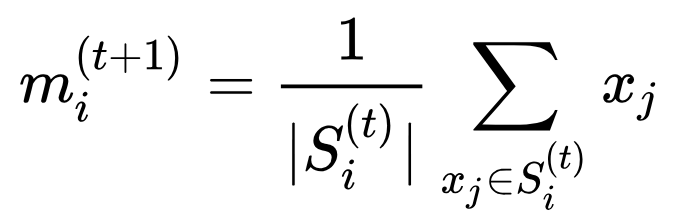
\includegraphics[width=0.3\textwidth]{update.png}
    \end{center}
    \vspace{-20pt}
\end{figure}

This continues until the algorithm converges, i.e. the true means of points in clusters equal the cluster centers.

\begin{figure}[!htb]
    \vspace{-10pt}
    \begin{center}
        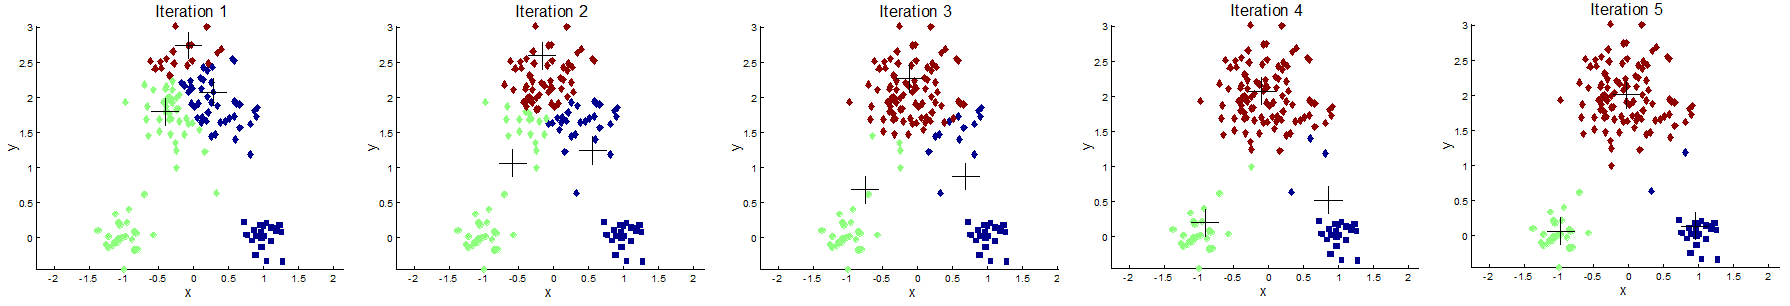
\includegraphics[width=1.0\textwidth]{iterations_flat.jpg}
    \end{center}
    \vspace{-20pt}
    \caption{Several iterations of k-means}
    \vspace{-20pt}
\end{figure}

\section{Other notes}

\subsection{Hyperparameters}
It's been noted that the $k$ in k-means stands for the number of clusters used in the algorithm. But how do we find this $k$? Usually, we just assume that we know this value, and just move on. It becomes a value that our algorithm doesn't actually need to figure out by itself, a parameter that originates externally (hence the name, \textbf{hyperparameter}) In reality, there exist several external algorithms that can calculate the optimum value of $k$, most of which involve running the clustering algorithm over multiple values of $k$, and using some kind of error measurement to see which ones performed better.

Likewise, the $K$ of KNN is a hyperparameter of the algorithm. It can be found in similar ways, the only major difference being that there is no rigorous "true" value that needs to be found, some values just inherently lead to better or worse performances.

You may have also noted that the choice of what kernel to use for an SVM is also a hyperparameter. This is usually a choice that depends on the nature of your data, much like choosing the right clustering algorithm to apply. The approach to finding the best kernel/algorithm typically involves matching up the type of data used to the algorithm that should perform best in theory, or running multiple algorithms to see which one performs best in practice.

\subsection{Overfitting}
\begin{wrapfigure}{r}{0.275\textwidth}
  \begin{center}
    \vspace{-45pt}
    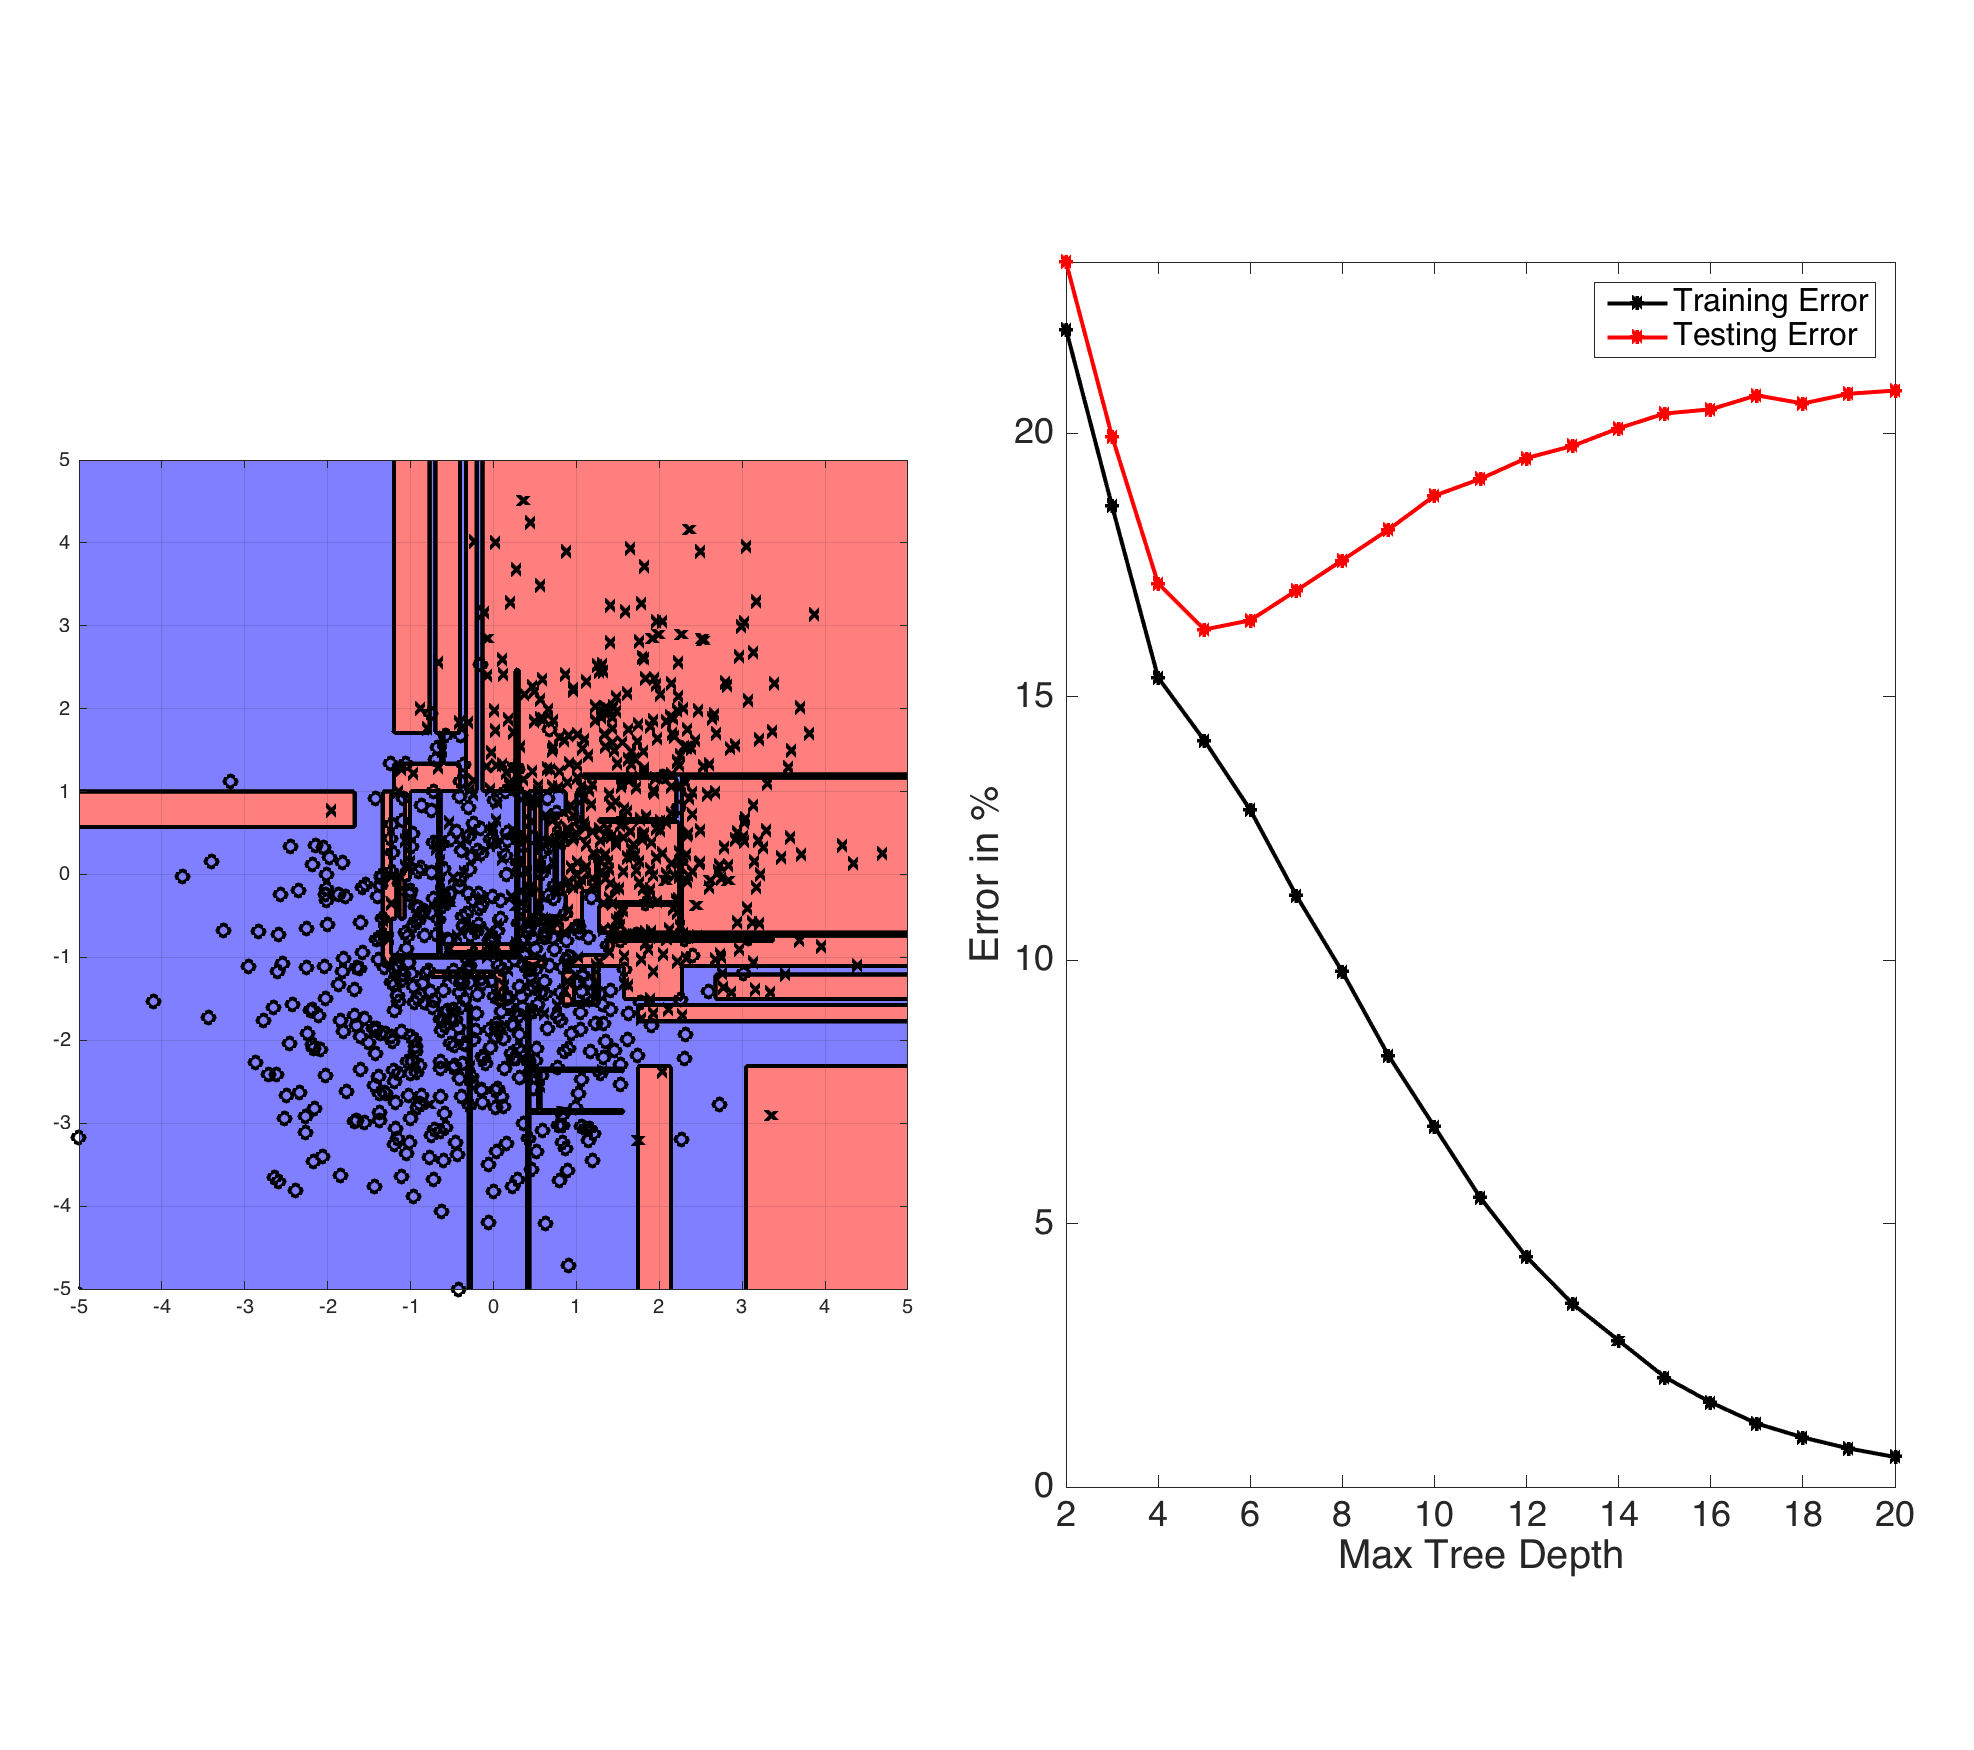
\includegraphics[width=0.275\textwidth]{overfit.png}
    \vspace{-40pt}
  \end{center}
  \caption{Overfitting a decision tree}
  \vspace{-10pt}
\end{wrapfigure}
You may have noted that decision trees can be expanded indefinitely, up until their accuracy becomes exactly 100.0\%. This may look good on paper, but the true performance of our network is actually much lower. What's worse, continuing to increase the accuracy \textbf{will actually decrease the true performance of the network}. In going for "perfect performance", our network will try to make irregular cuts around outliers, such as points located near a different cluster than their label. The issue is, new unlabeled points with the correct label are much more likely to land on this cutout, resulting in our attempt to correctly classify that one labeled point costing us a mislabeling of several unlabeled points. This problem is known as \textbf{overfitting}.

As hinted, the solution to the problem is just to stop training. A separate, unseen \textbf{testing} data set can be used to evaluate the performance after each iteration, and stopping optimization once it starts dropping. With decision trees, their depth can be limited to avoid absurd and greedy segmatations.

\subsection{Applications}
\begin{wrapfigure}{r}{0.25\textwidth}
  \begin{center}
    \vspace{-45pt}
    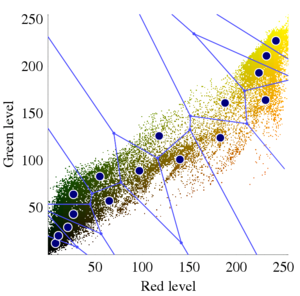
\includegraphics[width=0.25\textwidth]{quantization.png}
    \vspace{-30pt}
  \end{center}
  \caption{Color quantization through clustering}
  \vspace{-30pt}
\end{wrapfigure}
Even the simpler and more traditional ML algorithms can have a surprising amount of uses, some of them brilliantly surprising, plenty of them relating back to computer vision.

For example, clustering can be used in \textbf{color quantization}, a process somewhat similar to what we've done with quadtree compression. If given keypoints on a face, SVMs and decision trees can compare it against a known database and thus do \textbf{facial recognition}. If the only thing we have are some shuffled face images (extracted from Google Images, for example), a database could be created by passing said keypoints to our clustering algorithm.

\subsection{What to look forward to}
Next week we are going to discuss \textbf{neural networks}, which serve as the basis of Deep Learning. Keep in mind the linear way that decision trees and SVMs partition the feature space - it's very similar to how \textbf{artificial neurons} work, which are the very fundamental building block of neural networks, both the very simple ones, and the gigantic state-of-the-art prototypes.

It's those networks that enable us to better implement certain aspects of computer vision. Manually written image segmentation may fail on objects that have varying textures or color, or objects that blend in with their surroundings. This area has seen plenty of recent developments from the field of ML, large amounts of data and complex networks enabling us not only to \textbf{detect objects}, but even \textbf{classify} and \textbf{outline} them. Some other algorithms focus on tasks like \textbf{human pose estimation}, or \textbf{image captioning}. 
\begin{figure}[!htb]
    \vspace{-6pt}
    \begin{center}
        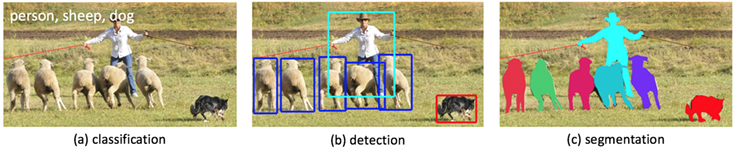
\includegraphics[width=0.8\textwidth]{ML_objects.jpg}
    \end{center}
    \vspace{-20pt}
    \caption{Various CV tasks done with ML}
    \vspace{-20pt}
\end{figure}

\end{document}